Powering most chemical manufacturing, heterogeneous catalysis is indispensable to the clean-energy transition and enables green hydrogen production, CO$_2$ valorization, and sustainable ammonia synthesis~\cite{norskov2011density}.
Computational catalyst discovery using density functional theory (DFT) calculations has substantially accelerated the discovery of promising catalytic materials relative to purely experimental trial-and-error. However, translating computational results into practical catalysts remains difficult due to the accuracy of the DFT simulations and the combinatorial complexity of catalyst surfaces~\cite{norskov2011density,ulissi2017toward}.
In every heterogeneous catalytic cycle, the adsorption of molecular species onto the catalyst surface is an elementary step whose energetics strongly influence catalytic activity and selectivity~\cite{norskov2011density,andersen2021adsorption} and determine the predictive power of microkinetic models and volcano plots that guide catalyst selection~\cite{norskov2011density}.
The accurate determination of the most stable adsorbate--surface configuration is thus a key in efficient computational catalyst discovery, from descriptor-based screening~\cite{norskov2011density,andersen2021adsorption} to high-throughput DFT workflows~\cite{greeley2017design,ulissi2017toward,yeo2021high,rosen2019identifying}.
However, configuration identification itself remains a persistent computational challenge. The configuration space grows combinatorially with surface complexity due to diverse site types (ontop, bridge, hollow, and their alloy variants), adsorbate orientations, and conformational flexibility. Consequently, the number of candidate configurations can easily exceed several hundred for a single polyatomic adsorbate on an intermetallic surface and scale into the thousands when co-adsorption or solvation effects are considered.

%Several approaches have been developed to address this combinatorial explosion issue, such as graph-theoretic approaches to systematically determine multidentate adsorption configurations on complex surfaces~\cite{deshpande2020graph} and machine learning (ML) frameworks that incorporate adsorbate chemical environment information to reduce the search space~\cite{ghanekar2022adsorbate}.
Traditional approaches to this combinatorial search problem each carry distinct trade-offs.
Exhaustive DFT enumeration over canonical site families~\cite{norskov2011density} is the most systematic but scales prohibitively: each DFT relaxation costs hundreds to thousands of CPU-hours, and a single surface can require $10^2$--$10^3$  evaluation cycles depending on adsorbate complexity.
Global optimization methods, such as genetic algorithms~\cite{vilhelmsen2014genetic}, basin hopping~\cite{wales1997global}, \emph{ab initio} random structure searching (AIRSS)~\cite{pickard2011ab}, and first-passage kinetic Monte Carlo~\cite{reuter2003first}, reduce the number of required evaluations through stochastic exploration, but still demand substantial expert oversight for convergence control, spin-state selection, and basis-set specification.
Since the number of candidate surfaces grows exponentially with alloying elements, the routine adsorption studies on a single surface can consume days of computational specialist. The high-throughput screening across composition space is also impractical without large enough computational resources~\cite{ulissi2017toward}.

The recent advances in machine learning force fields (MLFFs) have significantly reduced the computational needs for per configuration evaluations. Architectures such as MACE/MACE-MP~\cite{batatia2022mace,batatia2023foundation}, CHGNet~\cite{deng2023chgnet}, and EquiformerV2~\cite{liao2024equiformerv2} achieve near-DFT accuracy at orders-of-magnitude speedup, enabling relaxation of configurations that would be computationally impractical with DFT alone~\cite{lan2023adsorbml}. The releases of large-scale benchmark datasets, such as OC20 (Open Catalyst 2020)~\cite{chanussot2021open} and OC22 (Open Catalyst 2022)~\cite{tran2023oc22}, have also standardized evaluation protocols for adsorption energy prediction and catalyzed significant progress in MLFFs.
However, MLFFs solve only the \textit{fast energy and force evaluation} problem; they do not address the upstream \textit{search strategy} problem of deciding which configurations to evaluate among the combinatorially many possibilities.

Search strategies in computational materials science can be broadly categorized as \textit{open-loop} (policy fixed before evaluation, no adaptation based on results) or \textit{closed-loop} (each evaluation result feeds back into the policy, enabling adaptive exploration).
Most existing deep-learning approaches to materials prediction operate in an open-loop regime: graph neural networks trained to predict adsorption energies~\cite{reiser2022gnn} provide single-pass estimates without iterative refinement~\cite{chowdhury2018prediction}, and generative models for crystal structures~\cite{xie2022cdvae,zeni2025mattergen} propose candidates without incorporating relaxation feedback.
This architectural limitation implies these models cannot achieve the true absorption sites when their initial proposals miss stable configurations~\cite{abolhasani2023rise,yang2025stable}, and recent work has explicitly shown that active learning or similar feedback-driven strategies are required to efficiently navigate complex adsorption landscapes~\cite{yang2025stable}.
%Although focused on bulk crystal structure prediction, the GNoME project~\cite{merchant2023scaling} exemplifies both the promise and the fundamental ceiling of the open-loop paradigm: 2.2~million new crystal structures were discovered via GNN-guided screening, yet the pipeline cannot self-correct when its initial guesses fail, and the most stable structure for a given composition is not guaranteed to be among those proposed.
Prioritizing candidate configurations among combinatorially many possibilities requires \textit{chemical reasoning}, i.e., judgment about which binding motifs are plausible, which surface compositions favor specific adsorbate orientations, and when a predicted configuration is geometrically or chemically inconsistent.
Fixed open-loop computational pipelines are structurally incapable of providing this capability.

Large language models (LLMs) have emerged as natural candidates for this reasoning role, leveraging their ability to encode broad chemical knowledge and perform complex compositional reasoning \cite{mirza2024chembench,bran2024chemcrow,jablonka2023fourteen,ramos2025review}. Recent reviews have systematically surveyed the transformative impacts of LLM-driven scientific workflows across material discoveries, property predictions, and autonomous experiment designs \cite{jiang2025applications,miret2025enabling,ramos2025review}, especially the closed-loop autonomous systems. Platforms such as A-Lab \cite{szymanski2023alab}, ChemCrow \cite{bran2024chemcrow}, and Coscientist \cite{boiko2023autonomous} have demonstrated that feeding experimental or computational results back into the planning loop can let LLM agents coordinate multi-step chemical workflows and navigate large search spaces that previously required expert chemists \cite{zimmermann2025llm,yang2026quasar,stewart2026graphagents,chandrasekhar2026catalyst,weietal2025agentic}.

However, translating this closed-loop success to the adsorption configuration domain remains on a to-do list. Adsorb-Agent \cite{ock2026adsorbagent} recently took a pioneering step by coupling an LLM planner with EquiformerV2 \cite{liao2024equiformerv2} MLFF to generate adsorption hypotheses and enumerate candidates, effectively narrowing the search space relative to naive sweeps. Despite this progress, as an open-loop approach, Adsorb-Agent lacks systematic feedback from physical relaxations and cannot refine its reasoning.
The agent is never informed of whether its proposed configurations successfully reached the intended binding motifs or failed due to structural instability. 

The single-pass, open-loop regime of existing LLM agents might create three critical failures that become increasingly severe as surface complexity grows, including the reliability on LLM's initial site prediction, lack of interpretability of physical simulations, and LLM's systematic biased on certain sites.
% \textbf{(1) Reliability:} When the LLM's initial site prediction does not match any geometrically enumerable site on the surface, the system produces zero valid configurations and fails silently---with no mechanism to detect, diagnose, or recover from the error.
% \textbf{(2) Interpretability:} The system cannot distinguish a thermodynamically unstable binding site from a simulation failure, cannot flag dissociation or rearrangement events that produce misleading energy values, and cannot explain why a particular proposal succeeded or failed in physically meaningful terms.
% \textbf{(3) Much larger systematic bias:} We observe that current LLMs carry systematic biases---preferring high-symmetry sites, underweighting surface composition effects, and ignoring adsorbate conformational flexibility---that are impossible to anticipate through prompt engineering alone.
Without physical feedback, these biases propagate unchecked across every evaluation, systematically excluding potentially stable configurations.

These failure modes are inherent to any open-loop search strategy and motivate the same solution that active learning~\cite{settles2012active} and Bayesian optimization~\cite{snoek2012practical} have long validated, i.e., iteratively updating evaluation results back into the decision policy to guide subsequent proposals.
Recent work in autonomous materials discovery has further emphasized that closed-loop feedback is essential for reliable performance in complex search spaces~\cite{abolhasani2023rise,miret2025enabling}.

To overcome these limitations, we introduce \textbf{AdsMind} (\textbf{Ads}orption with \textbf{M}achine \textbf{I}ntelligence \textbf{\&} fee\textbf{d}back), a closed-loop multi-agent framework in which each MLFF relaxation result feeds back into the LLM planner, enabling the agent to detect, diagnose, and recover from its own reasoning errors (Figure~\ref{fig:pipeline}a).
% The framework closes the loop through three mechanisms in five agents: Chemical slip detection diagnoses mismatches between planned and realized configurations, FORBID constraints prevent retrying failed site families; and convergence-based early stopping avoids unnecessary computation (full architecture in Section~\ref{sec:methods}).
Through this closed-loop design, AdsMind realizes three properties that open-loop agents cannot achieve simultaneously: reliable convergence through error recovery (enabled by FORBID constraints), self-reflection through iterative use of relaxation feedback, and interpretability through physically grounded feedback artifacts (enabled by Chemical Slip detection).

We evaluate AdsMind across 82 surfaces (20 in CMU20 and 62 in OCD-GMAE62 benchmarks) with four LLM backends and MACE-MP-0 FF, benchmarking against conventional baselines and the open-loop agent Adsorb-Agent~\cite{ock2026adsorbagent}.
DFT validations using VASP\cite{kresse1996efficient} with Perdew--Burke--Ernzerhof (PBE) exchange-correlation functional~\cite{perdew1996generalized} and projector augmented-wave (PAW) pseudopotentials on six representative systems in CMU20 dataset reveal that the open-loop baseline produces qualitative sign errors on molecular adsorbates, while AdsMind preserves 100\% sign-correctness with competitive quantitative agreement.
Systematic comparison with broader sampling strategies further delineates the reliability--depth--relaxation-budget trade-off, establishing the complementary niches of closed-loop refinement and depth-maximizing search---defining the operating envelope in which this architecture adds value.
By delivering reliability, self-reflection, and interpretability simultaneously, AdsMind establishes a foundation for autonomous adsorption configuration search.


\begin{figure}[t]
    \centering
    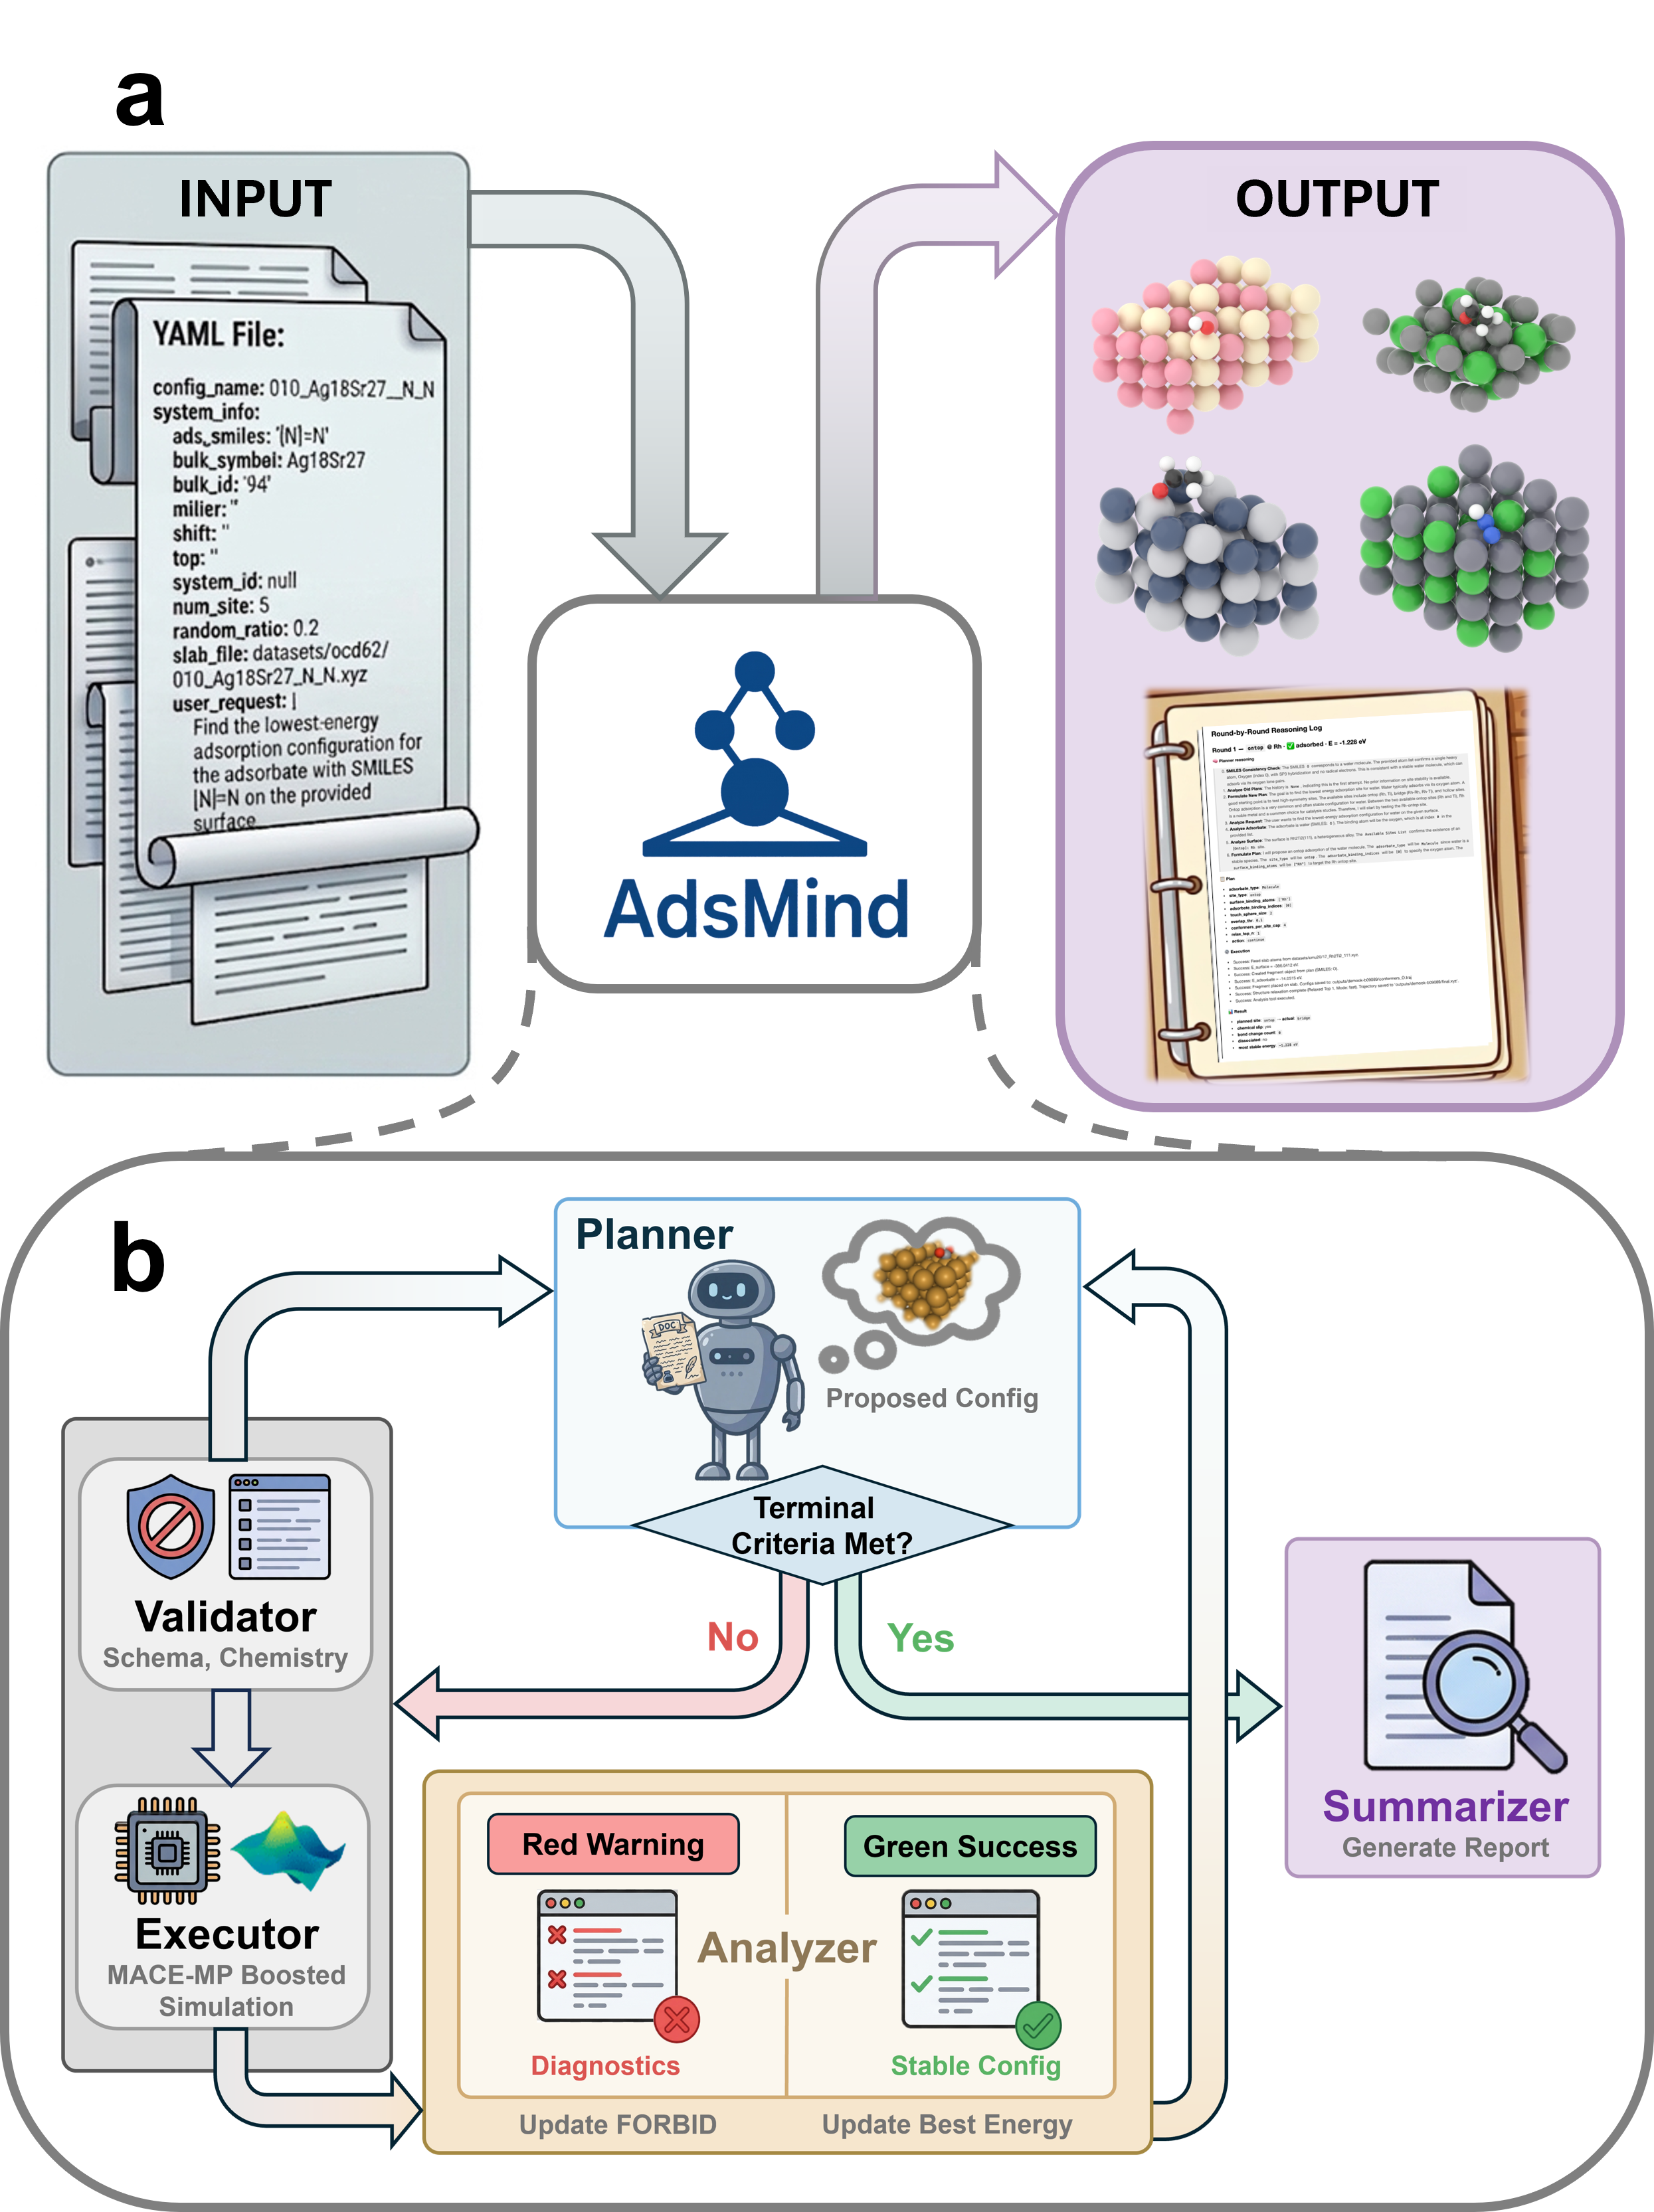
\includegraphics[width=0.5\linewidth]{images/figure1_pipeline.png}
    \caption{\textbf{Overview of AdsMind.} (a) Schematic diagram of the AdsMind closed-loop multi-agent framework, showing the Planner, Validator, Executor, Analyzer, and Summarizer agents. (b) Test benchmark datasets: CMU20 (20 surface-adsorbate cases) and OCD-GMAE62 (62 oxide, intermetallic, monometallic, and compound surfaces across two testing tiers).}
    \label{fig:pipeline}
\end{figure}
